\chapter{Evaluierung}
\label{chp:Evaluation}
  \citet{distrh2} haben gezeigt, dass deren paralleler Ansatz sehr nah an die optimale parallele Effizienz von $\mathcal{O}(\frac{nk}{p})$ herankommt, falls $n$ deutlich größer als $p$ ist.
  Im folgenden gilt es diese Argumentation auf den vorliegenden Algorithmus zu übertragen und durch Daten aus praktischen Laufzeitmessungen zu unterstützen.
  
  \section{Theoretische Abschätzung}
  
  \begin{ann}
  \label{ann:nodes}
    Es existiert $q \in \N$ sodass für $p := \left| \Proc \right|$ gilt:
    \[ p = 2^q \]
  \end{ann}
  Diese Annahme wurde bereits bei der Vorstellung des Algorithmus getroffen.
  
  \begin{ann}
  \label{ann:tree}
    Die ersten $q$ Ebenen des Clusterbaumes $T_\Omega$ bilden einen vollständigen Binärbaum.\\
    Es existiert eine Konstante $C_{st}$, sodass für alle Teilbäume $T_{sub}$ mit $\tau := root(T_{sub}) \in T_\Omega^{(q)}$ gilt
    \[
     depth(T_{sub}) \leq C_{st} \frac{n}{kp} \text{ und}
    \]
    \[
     |\tau| \leq C_{st}\frac{n}{p}
    \]
  \end{ann}
  Diese Annahme wurde durch die Wahl der Abbruchbedingung bei der Konstruktion des Clusterbaumes sichergestellt. Es gilt sogar $depth(T_{sub}) = \log_2(\frac{n}{p}) - \mathfrak{l}$ (vgl. \autoref{eq:l}),
  da jeder Prozess gerade einen Teilbaum konstruiert, wie er zuvor vom gesamten nicht-parallelisierten Algorithmus vorgenommen wurde (vgl. letzter Absatz in \autoref{sec:data}). Zwar lässt sich die
  Anzahl Elemente der Cluster $\tau \in T_\Omega^{(q)}$ nicht exakt angeben, da die Unterteilung in Sohncluster nicht nach Kardinalität vorgenommen wird, jedoch beträgt diese im Schnitt gerade 
  $\frac{n}{p}$. Die Konstante $C_{st}$ kann also als $\approx 1$ angenommen werden.
  
  Die Methode \code{_setup(Cluster *c, int depth)}, die in unserem Algorithmus die Verteilung der Cluster auf Prozesse vornimmt, gewährleistet folgende Eigenschaften:
  
  \begin{lem}
    (Zuständigkeiten)\\
    Für den verteilten Clusterbaum $T_\Omega$ gelten folgende Eigenschaften:
    \begin{equation}
      \text{Für } \tau \in T_\Omega^{(\geq q)} \text{ existiert genau ein } P \in \Proc \text{ mit } \tau.\tcode{activ} = id_P.
    \end{equation}
    \begin{equation}
      \text{Jeder Prozess } P \in \Proc \text{ berechnet auf jeder Ebene } T_\Omega^{(q')}, \ q' \in \nullhaken{q-1} \text{ genau eine Transfermatrix.}\label{eq:log}
    \end{equation}

    Aus \autoref{eq:log} folgt direkt mit $q = \log_2 p$ (vgl. \autoref{sec:work}):
    \begin{equation}
      \text{Die Anzahl Transfermatrizen } E_\tau, \ \tau \in T_\Omega^{(\leq q)} \text{ pro Prozess beträgt } q.\tag{\ref{eq:log}'}
    \end{equation}
  \end{lem}

%   Um den Speicherbedarf abschätzen zu können, verlassen wir uns auf das von \citet{sparsity} vorgestellte Konzept der \textit{sparse partitions} (deutsch etwa ``seltene Partitionen''). 
%   \begin{ann}
%     (Seltenheit)\\
%     Seien für alle Cluster $\tau \in T_\Omega$
%     \begin{align*}
%       row(\tau) &:= \{\sigma \in T_\Omega \ | \ \tau \times \sigma \in T_{\Omega \times \Omega} \},\\      
%       col(\tau) &:= \{\sigma \in T_\Omega \ | \ \sigma \times \tau \in T_{\Omega \times \Omega} \}.
%     \end{align*}
%     Wir nehmen im folgenden eine von $n$, $p$ und $k$ unabhängige Konstante $C_{sp} \in \N$ (vgl. \citet{sparsity}) an, sodass für alle $\tau \in T_\Omega$ gilt:
%     \[
%       \left| row(\tau) \right| \leq C_{sp},\ \ \left| col(\tau) \right| \leq C_{sp}.
%     \]
%   \end{ann}

  Da wir einen parallel arbeitenden Algorithmus haben ist es für die Abschätzung des Rechenaufwandes nicht ausreichend die Anzahl an Operationen zu zählen. Da die Prozesse kommunizieren müssen ist 
  regelmäßig eine Synchronisation der Prozesse notwendig. So wird vorkommen, dass ein Prozess $P_i$ schneller seine Berechnungen durchführt als ein Prozess $P_j$ und dann auf diesen warten muss bevor
  die Kommunikation stattfinden kann. 
  
  Daher verwenden wir einen ähnlichen Ansatz, wie er auch beim BSP-Modell \citep{bsp} verwendet wurde: Die gesamte Berechnung wird in eine Sequenz von $s \in \N_0$ \textit{Superschritten} eingeteilt,
  die jeweils unabhängig von den anderen Prozessen von einem Prozess durchgeführt werden können. Der $i$-te Superschritt startet simultan, sobald alle Prozesse den $i-1$-ten Superschritt abgeschlossen
  haben, $i \in \haken{s}$. Als Zeiteinheit verwenden wir die abstrahierte Einheit \textit{Zyklus}. Ein Zyklus sei dabei lang genug um eine arithmetische Operation, einen Speicherzugriff oder eine Sende-
  oder Empfangsoperation für einen \code{double}-Wert durchzuführen.
  
  Da der Algorithmus mit einer impliziten $\mathcal{H}^2$-Matrix arbeitet, beschränkt sich die Konstruktion auf den Clusterbaum.
  
  \begin{lem}
    (Konstruktion)\\
    Die Konstruktion des Clusterbaumes benötigt $\mathcal{O}(n)$ Zyklen.
  \end{lem}
  
  ...
  
  \section{Laufzeitmessung}
  Um Laufzeitdaten des Algorithmus zu sammeln, wurde dieser auf dem NEC HPC-Linux-Cluster der CAU Kiel ausgeführt. Jeder Knoten dieses Clusters ist mir 192 GB Arbeitsspeicher und zwei Intel Xeon Gold 
  6130 bestückt, die einen Kerntakt von 2,1 GHz aufweisen. Verbunden sind die Knoten über EDR infiniband. Als Compiler wurde der Intel-C-Compiler 17.0.4, sowie der Intel-MPI-Compiler 17.0.4 verwendet.
  
  Es wurden unterschiedliche Testreihen durchgeführt. Es wurden jeweils entweder die Anzahl Prozesse oder die Anzahl Sonnen verändert, um beide Ansätze unabhängig voneinander testen zu können.
  In den ersten beiden Testreihen wurde die Anzahl Sonnen bei konstanter Anzahl Prozesse variiert. Die Messergebnisse sind in \autoref{fig:1-32x} sowie in \autoref{tab:1-32x} 
  aufgeführt.
  
  \begin{figure}[t]%
  \centering
  \begin{subfigure}{\textwidth}
    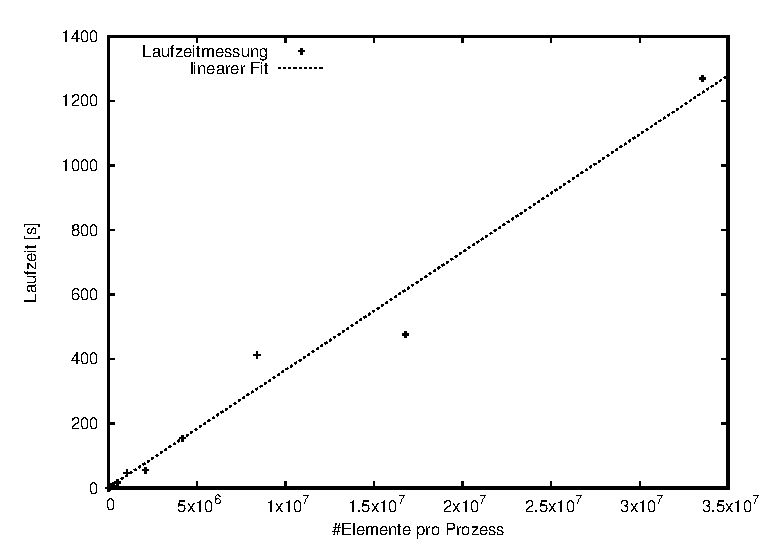
\includegraphics[width=0.8\textwidth]{img/grav1_lin.eps}
    \subcaption{Dieser Testlauf wurde mit $p = 1$ durchgeführt und entspricht damit der nicht-parallelen Variante.}
  \end{subfigure}
  \begin{subfigure}{\textwidth}
    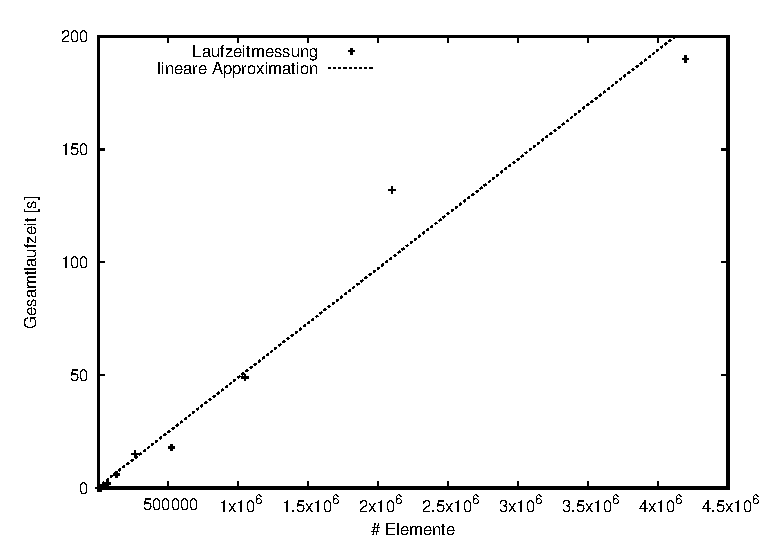
\includegraphics[width=0.8\textwidth]{img/grav_32_lin.eps}
    \subcaption{Dieser Testlauf wurde mit $p = 32$ durchgeführt, genau ein Knoten des Rechenclusters auszulasten.}
  \end{subfigure}
  \caption{In dieser Abbildung ist der Zusammenhang der Laufzeit mit der Anzahl an Elementen pro Prozess dargestellt.}
  \label{fig:1-32x}
\end{figure}
  
  \blindtext
  
  \begin{table}[t]
 \begin{subtable}{0.45\textwidth}
  \begin{tabular}{c c c}
    \ \ \ \ 
    &
    \begin{tabular}{|P{2cm}|P{2cm}|}
      \hline
      \#Elemente \newline pro Prozess & Laufzeit [s] \\
      \hline
      $2^{10}$ & 0,008324 \\
      $2^{11}$ & 0,02569 \\
      $2^{12}$ & 0,04406 \\
      $2^{13}$ & 0,1348 \\
      $2^{14}$ & 0,503 \\
      $2^{15}$ & 0,6866 \\
      $2^{16}$ & 1,905 \\
      $2^{17}$ & 5,271 \\
      $2^{18}$ & 6,454 \\
      $2^{19}$ & 17,52 \\
      $2^{20}$ & 46,63 \\
      $2^{21}$ & 55,57 \\
      $2^{22}$ & 154,5 \\
      $2^{23}$ & 413,1 \\
      $2^{24}$ & 476 \\
      $2^{25}$ & 1270 \\
      \hline
    \end{tabular}
    &
    \ \ \ \ 
  \end{tabular}
 \subcaption{Dieser Testlauf wurde mit $p = 1$ durchgeführt und entspricht damit der nicht-parallelen Variante.}
 \end{subtable} \ \ 
 \begin{subtable}{0.45\textwidth}
  \begin{tabular}{c c c}
    \ \ \ \ 
    &
    \begin{tabular}{|P{2cm}|P{2cm}|}
      \hline
      \#Elemente \newline pro Pozess & Laufzeit [s] \\
      \hline
      $2^{10}$ & 0,02877 \\
      $2^{11}$ & 0,06701 \\
      $2^{12}$ & 0,1962 \\
      $2^{13}$ & 0,3097 \\
      $2^{14}$ & 0,7803 \\
      $2^{15}$ & 2,402 \\
      $2^{16}$ & 3,288 \\
      $2^{17}$ & 8,54 \\
      $2^{18}$ & 19,9 \\
      $2^{19}$ & 27,01 \\
      $2^{20}$ & 65,41 \\
      $2^{21}$ & 170 \\
      $2^{22}$ & 239,1 \\
      $2^{23}$ & 580,4\\
      & \\
      & \\
      \hline
    \end{tabular}
  \end{tabular}
 \subcaption{Dieser Testlauf wurde mit $p = 32$ durchgeführt, um genau ein Knoten des Rechenclusters auszulasten.}
 \end{subtable}
\caption{In dieser Tabelle sind die Laufzeitmessungen der ersten beiden Testläufe aufgeführt.}
\label{tab:1-32x}
\end{table}
